% !TEX root = nips_2018.tex

\section{Conditioning Declares Knowledge}\label{condknow}

Physics is rife with problems which benefit from both declarative and generative knowledge.
For example, inferring 3D structure from 2D measurements requires prior beliefs about 3D geometry.
Encoding knowledge about the world such as `rigid objects do not intersect' would bring our prior closer to reality and help make better inferences.  One way to encode this knowledge
would be to try to construct a family of distributions such that the objects never get placed in overlapping places. However, this approach requires careful manipulation of the prior.
If the prior is highly parameterized (such as a deep neural network) there is no mechanism for constructively encoding this knowledge into the prior.
In figure \ref{fig:nointersect} we show how with the appropriate language support and inference algorithms, this knowledge can be conditioned on directly.

\begin{figure}[h]
\centering
\begin{minipage}[t]{5cm}
\centering
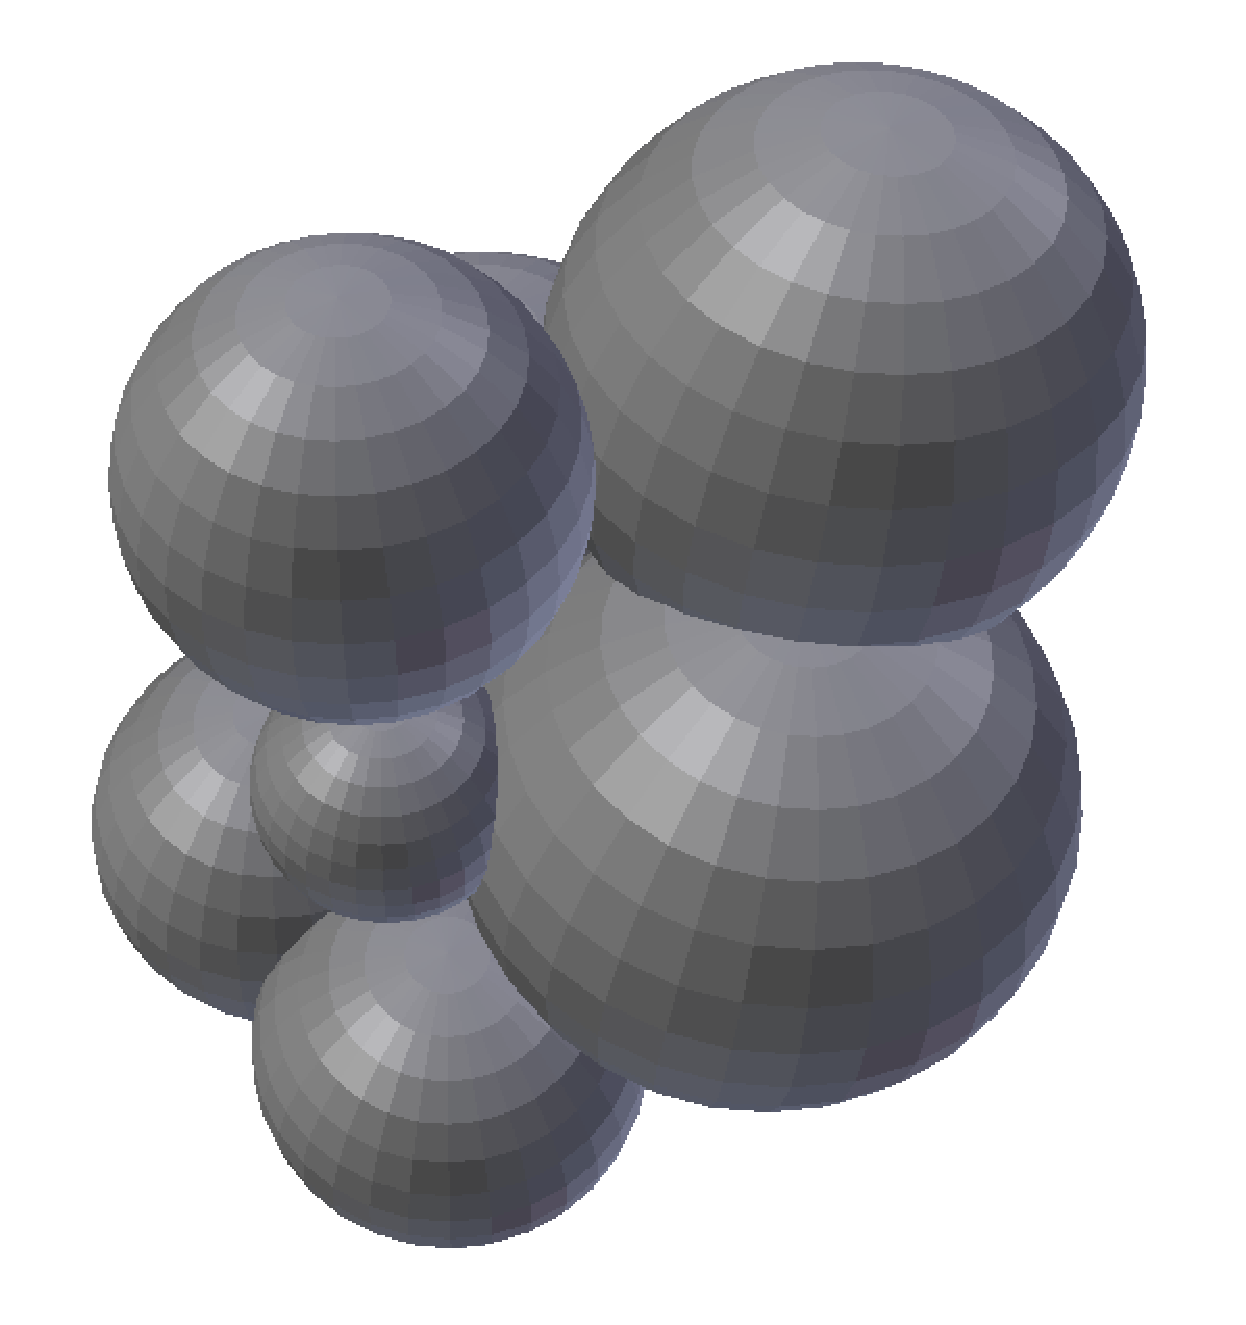
\includegraphics[width=0.5\linewidth]{figures/clunk}
\begin{verbatim}
        rand(objs)
\end{verbatim}
\end{minipage}%
\begin{minipage}[t]{5cm}
\centering
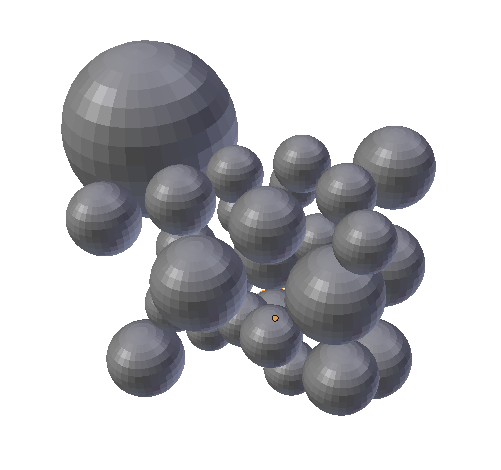
\includegraphics[width=0.8\linewidth]{figures/render}
\begin{verbatim}
pred = nointersect(objs)
rand(scene, pred)
\end{verbatim}
\end{minipage}%
\begin{minipage}[t]{5cm}
\centering
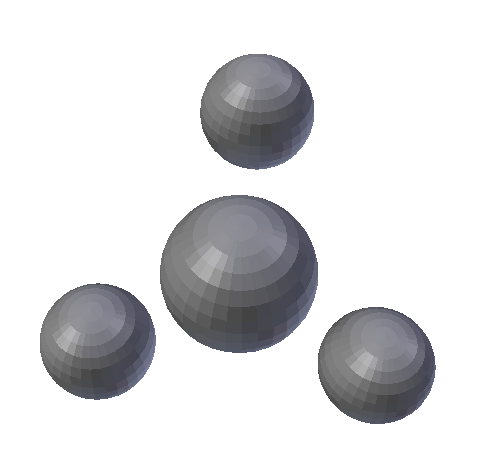
\includegraphics[width=0.5\linewidth]{figures/equi}
\begin{verbatim}
pred = equidistant(objs)
rand(scene, pred)
\end{verbatim}
\end{minipage}
\caption{A weak prior (left) does not respect rigid body constraints on objects, whereas (center) is conditioned on the predicate that objects don't intersect.  (right) objects are conditioned on being equidistant, resulting in a tetrahdral arrangement}
\label{fig:nointersect}
\end{figure}

% \begin{figure}[!htb]
% \begin{minipage}
% 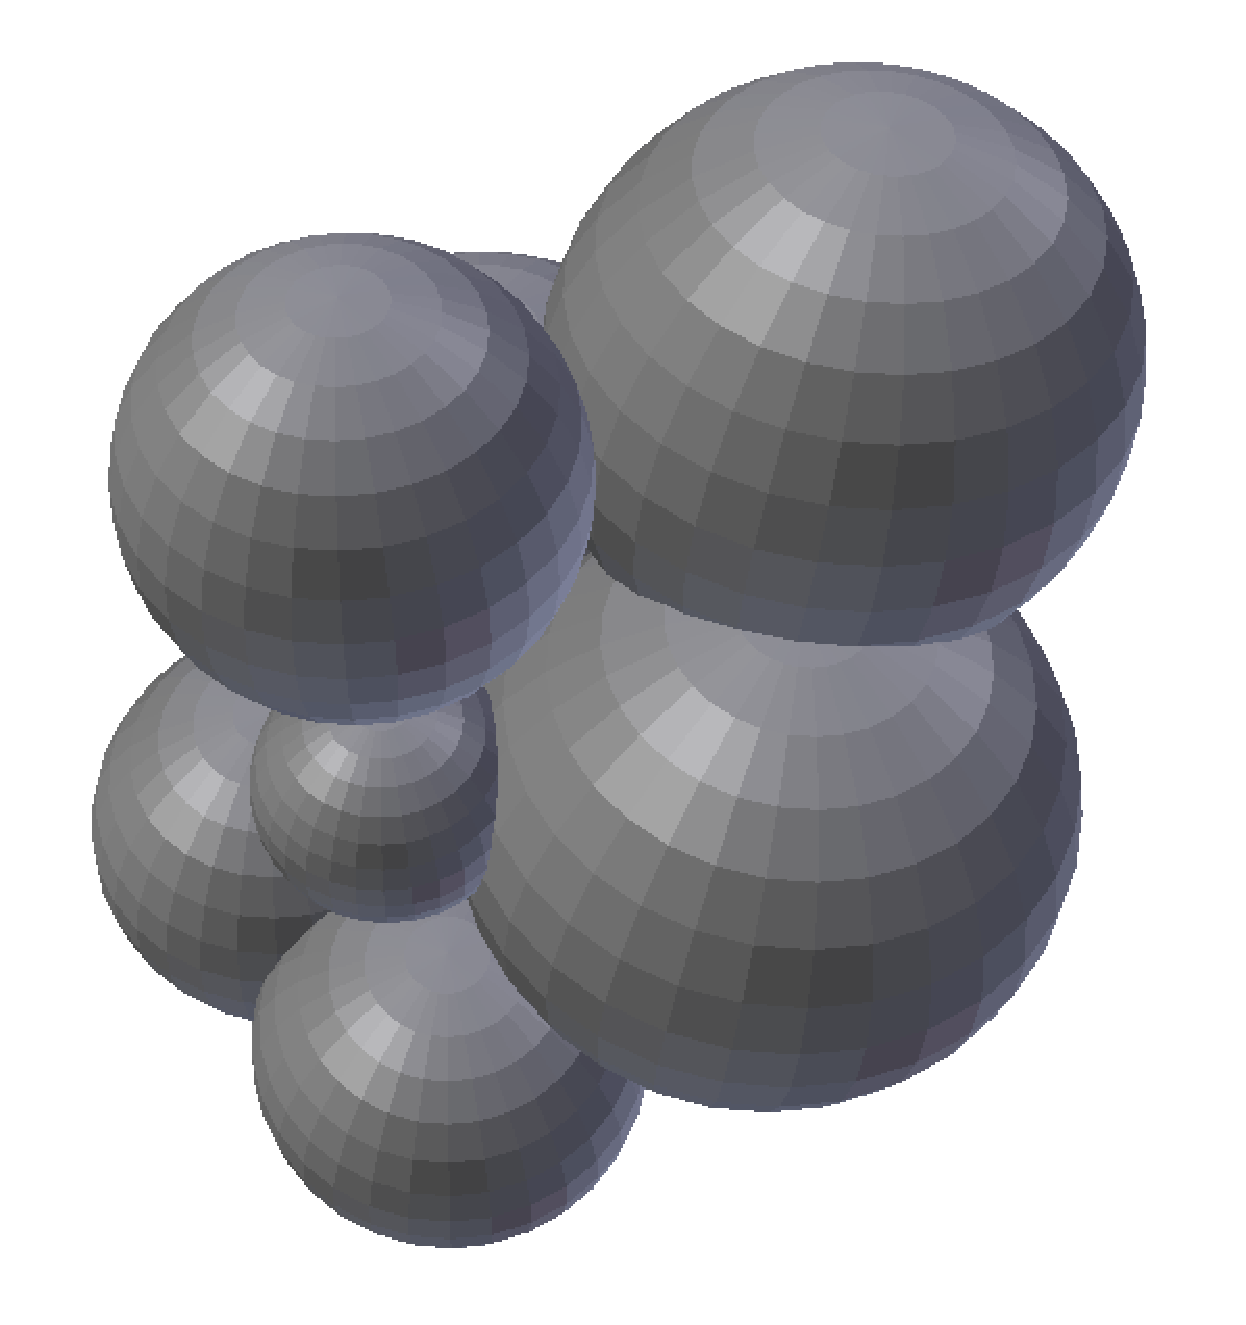
\includegraphics[width=0.3\linewidth]{figures/clunk}
% \end{minipage}
% 	\centering
%   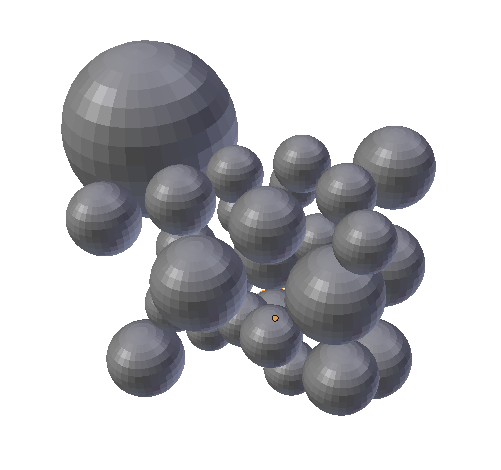
\includegraphics[width=0.3\linewidth]{figures/render}
%   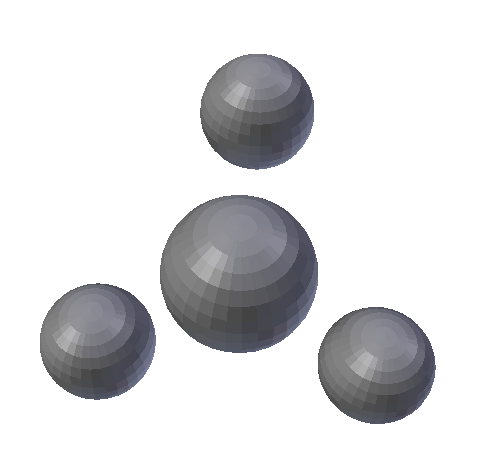
\includegraphics[width=0.3\linewidth]{figures/equi}
% 	\caption{A weak prior (left) does not respect rigid body constraints on objects}
% 	\label{fig:rcd}
% \end{figure}

% An alternative approach would be to declare this knowledge directly to any family of models by conditioning. Conditioning provides knowledge by creating constraints that a distribution must satisfy.
% For example, in a latent variable model with latent variable $z$ and observation
% $x$, the posterior distribution conditional on an observation $x^*$,
% $p(z \g x = x^*)$, enforces that samples be consistent with the observed data
% --- it declares knowledge about $x$ in the form of the observed data.

% Returning back to the probabilistic renderer, we can use conditioning to 
% declare the knowledge that objects do not overlap without having to understand the internals
% of the specific render. Let ${o_1, ..., o_n}$ be solid objects
% which we would like to appear in the scene, and $p(r \g {o_1, ..., o_n})$
% be any rendering model. Then consider $p(r \g {o_1, ..., o_n})$ 
% conditional on $r(o_i) \cap r(o_j) = \emptyset$.
% By construction, samples from $p(r \g {o_1, ..., o_n}, r(o_i) \cap r(o_j) = \emptyset)$ can only
% produce renders where the objects do not overlap. In this sense, 
% condition declares knowledge via constraints the joint distribution must satisfy.
It is possible in existing probabilistic languages to encode such knowledge.
Figure \ref{fig:compare} shows the predicate which asserts no intersection in both WebPPL, and our contribution, Omega.
\begin{figure}[h]
\centering
\begin{minipage}[c]{5.7cm}
\begin{Verbatim}
function nointersect(s1, s2)
  d1 = d(s1, s2)
  d2 = s1.radius + s2.radius
  d1 < d2
end
\end{Verbatim}
\end{minipage}%
\begin{minipage}[c]{5.7cm}
% \centering
\begin{Verbatim}
var geq = function(lhs, rhs) {
  factor(min(lhs - rhs, 0)) }
var nointersect = function(s1, s2) {
  d1 = d(s1, s2)
  d2 = (s1.radius + s2.radius)
  return geq(d1, d2) }
\end{Verbatim}
\end{minipage}%
\caption{A comparison of the no-intersection condition in Omega WebPPL. Omega conditions directly on the predicate while WebPPL incorporates a factor into the model.}
\label{fig:compare}
\end{figure}

% . We can build a 
% distribution over weights and heights by building
% a distribution over heights then a distribution of weight given height
% $(p(h) p(w \g h))$. However, a generic model does include the knowledge
% we have that taller people tend to weigh more. One way to include this
% knowledge would be to place prior on the distribution of weights given heights
% that enforces a positive relationship.

% Suppose that we are given accurate models, probability distributions, for the
% heights and weights of humans, but we do not know how weights and heights
% are related. 



% Denote these probability distributions
% as with parameters $\theta$ as p(h ; \theta_h)$ and $p(w ; \theta_w)$.


% Consider models probability distributions for the heights and weights 

\paragraph{Random Variables.} Probability models lie on top of probability
spaces. A probability space is a measure space $(\Omega, {\cal H}, {\cal P})$,
where ${\cal H}$ is a sigma algebra and ${\cal P}(\Omega) = 1$ \citep{ccinlar2011probability}. Random variables are
functions from the space $\Omega$ to a realization space ${\cal X}$. As a concrete 
example the space $\Omega$ can be thought of as a hypercube, with ${\cal P}$ being
uniform over that hypercube. To build a normal random variable, we need a function
that maps from $\Omega \to \mathbb{R}$. If the underlying probability space is uniform, then
this function is the inverse cumulative distribution function of the normal. 

A \emph{model} $\cM$ is a collection of random variables along with a probability space. 
For example, a probabilistic
graphical model defines a group of random variables via their conditional independencies.
To fully specify a model, we need both the measure space and the
collection of random variables on which it acts.

\paragraph{Conditioning Creates New Models.}
Conditioning a model
creates a new model. As a simple example consider a model $\cM$ with two
random variables $X_1$ and $X_2$ that both take real values. Conditioning
$\cM$ on $X_1 = 1$, defines a new model based on limiting the measure space
$\Omega$ to only the set $A = \{ \omega : X_1(\omega) = 1\}$. 
The new model $\cM^*$ can be defined with probability space
\begin{align*}
(\Omega \cap A, \{A \cap B, B \in {\cal H} \}, {\cal P} / {\cal P}(A)) 
\end{align*}
with the same random variables $X_1$ and $X_2$.\footnote{We defer issues of 
conditioning on events of measure zero.} Sampling from $M^*$ produces 
samples only where $X_1 = 1$ thereby producing a model that respects the 
knowledge that $X_1 = 1$. Note, the new probability measure comes
from the conditional probability measure.

More generally, conditioning on any predicate defines a new model. These
predicates can include comparisons between random variables and general 
functions of them. Example predicates include 
comparisons $X_i < X_j$, transformations $\exp(X_i) > 2$, and restrictions $X_i < 0$.
Given
a model $\cM$  with probability space $(\Omega, {\cal H}, {\cal P})$ and
random variables $X_1,\dots, X_n$ with predicate $d(X_1, \dots, X_n) \in \{0, 1\}$,
we can build a new model by restricting the probability space to the subset of
$\Omega$ that make the predicate true (takes value 1). This model
is defined exactly as above.  Let $A = \{\omega : d(X_1(\omega), \dots, X_n(\omega)) = 1\}$,
then $\cM^*$ has probability space
\begin{align*}
(\Omega \cap A, \{A \cap B, B \in {\cal H} \}, {\cal P} / {\cal P}(A)),
\end{align*}
where the random variables $X_1,...X_n$ remain unchanged. Sampling from
the model $M^*$ generates $X_1, ..., X_n$ where the predicate $d$ is true.
Thus, conditioning on a predicate creates a new model with the same 
random variables that enforces the predicate's truth 
without having to redefine random variables. In this sense conditioning
creates new models that respect knowledge (e.g. objects in a 3D render 
can't intersect) without having to alter or understand the random variables (rendering functions).

The general construction of new models might require conditioning
on sets of measure zero. This process can be made rigorous
via disintegration \citep{chang1997conditioning}. Disintegration can
be thought of as the reversal of building joint distributions through
product measure constructions.

% When building models with prior beliefs via conditioning, we would like
% the property that given an infinite collection of observations, the 
% posterior predictive distribution converges to true sampling distribution.
% To study this, consider a model with two random variables that are independent,
% $X_1$ is a function of $\omega_1$ and $X_2$ is a function of $\omega_2$. Suppose
% that the true sampling distribution has $X_1$ and $X_2$ positively correlated.
% For the prior beliefs to support positive correlations, we 
% could condition on a prior belief that $X_1$ and $X_2$ are close. However
% if the form of the closeness isn't controlled by a random variable, observing
% an arbitrary amount of data from the true distribution will not change
% the dependence between $X_1$ and $X_2$ in the model. 
% \begin{align*}
% X_j^*(\omega^*) = \sigma(f_\Beta(X_{j, 1}, ..., X_{j, n})) > b, \\
% \end{align*}
% Conditioning on $X_j^*$ produces a new set of models that have 
% dependence between . Knowledge is encoded in the prior distribution
% on $\Beta$. If $f_\Beta$ has priors over the true dependence between
% $X_{., 1},...,X_{., m}$, then this new model family will converge
% to the true underlying distribution.

% rr: TODO the above can me made into a proof

% \subsection{Bayesianism vs. Bayesian Computation}
% The way we 


% \section{Higher Order Random Variables}
% People often entertain beliefs about probability statements. For instance most people accept 
% trust expert-given odds that a particular sports team will win a tournament, 
% or politician will win an election, more than the odds of those given by non-experts.
% The apparent failure of probabilistic expressions to distinguish 
% between these cases led to alternative formalisms of uncertainty \citet{Shampher}, 
% but within the probabilistic framework both \citet{Pearl} and \citet{Hyberg} demonstrated 
% that such higher order distributions were induced from the original model, no new machinery was needed.

% As a concrete example of this, suppose we have a stochastic 
% dynamical system model of human blood glucose 
% controlled by some 
% parameters $\Theta$ with a prior. A priori we know that the average blood pressure 
% in a person lives in a physically plausible range $40-400$. A way to
% encode this would be to change the prior on the parameters $p(\Theta)$ 
% to so that any sample from that prior yields has average in the physically
% plausible range. This can be challenging because it requires a detailed
% understanding of the stochastic dynamical system. 

% Alternatively, we could try to take the conditioning approach from the
% previous section. But conditioning in the previous section required explicitly
% defined random variables, and while the average glucose is a random variable
% because the parameter $\Theta$ is random, it is not an explicit random variable.
% The scenario requires the ability to both define and condition on 
% probability distributions over either random variables or properties of 
% random variables (e.g. expectations).
% In this section we introduce the random conditional 
% distribution ($\randcond$) to support this task.

% \paragraph{The Random Conditional Distribution.}
% The random conditional distribution of $X$ given $\Theta$ -- which we denote $\rcd(X, \Theta)$ or $\rcdxy{X}{\Theta}$ -- is a random distribution: a random variable which takes values in the domain of random variables.
% Informally, $\rcdxy{X}{\Theta}$ is a function of $\omega$ that returns functions of $\omega$
% of the same type as $X$. Formally, $\rcd$ is a distribution over conditional random variables:

% % The primary mechanism for conditioning is $\cond$, which constructs conditional random variables:
% % \begin{definition}
% % Let $X:\Omega \to T$ be a random variable, $Y$ an indicator function, and $\conds{X}{Y}: \Omega_{|Y} \to T$ be a conditional random variable defined as: $X_{|Y}(\omega) = X(\omega)$.
% % $X_{|Y}$ is defined on a conditioned probability space $(\Omega, \Sigma, \mu_{|Y})$ where $\mu_{|Y}$ is a conditional measure: $
% % \mu_{|Y}(A) = \mu(A \cup Y^{-1}(\{1\})) / \mu(Y^{-1}(\{1\})$.
% % % That is, $\cond: (\Omega \to T) \times (\Omega \to \{0, 1\}) \to (\Omega \to T)$ is a operator that restricts the domain of $X$ to those inputs consistent with $Y$.
% % \end{definition}


% \begin{definition}The random conditional distribution of a random variable $X: \Omega \to T_1$ given $\Theta: \Omega \to T_2$ is a random variable $\rcdxy{X}{\Theta}: \Omega \to (\Omega \to T_1)$, defined as:
% \begin{equation}\label{eq:rcd}
% (\rcdxy{X}{\Theta})(\omega) = [\conds{X}{\Theta = \Theta(\omega)}]
% \end{equation}
% \end{definition}
% For example if $\Theta = \bern(0.4)$ and $X = \normal(\Theta, 1)$, then $\rcdxy{X}{\Theta}$ is a random distribution 
% whose domain comprises of two normal distributions $X_1 = \conds{\normal(\Theta, 1)}{\Theta = 1}$ and $X_2$.
% The probabilities of $X_1$ and $X_2$ with respect $\rcdxy{X}{\Theta}$ are determined by the prior probabilities of the different outcomes of $\Theta$: $P((\rcdxy{X}{\Theta}) = X_1) = 0.4$ and $P((\rcdxy{X}{\Theta}) = X_2) = 0.6$.

% A random conditional distribution is most useful in combination with other functions.
% Expectation is perhaps the most important example, which when composed with $\rcd$ produces conditional expectation.
% Restricting to real valued variables, expectation $E$ is a functional that maps a random variable to a real value
% (($\Omega \to \mathbb{R}) \to \mathbb{R}$).
% When $X$ is a real valued random variable, $\rcdxy{X}{\Theta}$ is not real valued, and hence not a valid argument to $E$.

% However, just as arithmetic operations such as $+$ and $-$ extend from the domain of numbers to the domain of random variable (pointwise $X + Y = \omega \mapsto X(\omega) + Y(\omega)$), $E$ extends from the domain of random variables to the domain of random variables over random variables in precisely the same way.
% % Since random variables are themselves functions, $E$ is an operator, functional or more generally a higher-order function.  
% % As described in section X a function with domain $T$ can be lifted to a functional of $T$-valued random variables.
% % $T$ is purposefully left abstract, because in addition to lifting functions defined on the reals etc, we can lift functions defined on random variables.
% % Expectation is a cannonical example of a random variable valued function, with type $E : (\Omega \to \mathbb{R}) \to \mathbb{R}$.
% That is, $\ee$ has a lifted counterpart $\lifted{\ee} = \lift(\ee)$ with type $\lifted{\ee} : (\Omega \to (\Omega \to \mathbb{R})) \to (\Omega \to \mathbb{R})$, which maps a distribution over real valued random variables to a distribution over real values (expectations).
% % $$
% % \lifted{\ee}(X)(\omega) = \mean{X(\omega)}
% % $$
% The operator $\rcd$ composed with $\ee$ constructs conditional expectation (with respect to a random variable $\Theta$):
% \begin{equation}
% \lmean{\rcdxy{X}{\Theta}} = \lmean{\omega \mapsto \conds{X}{\Theta = \Theta(\omega)}} 
%                     = \omega \mapsto \mean{\conds{X}{\Theta = \Theta(\omega)}}\\
% \end{equation}
% The final term $\omega \mapsto \mean{\conds{X}{\Theta = \Theta(\omega)}}$ matches the definition of
% conditional expectation
% with respect to a random variable $\mean{(X\mid \sigma (Y))(\omega)} = \mean{X \mid Y = Y(\omega))}$.
% That is the conditional expectation is a random variable with randomness provided by the conditioning set.

% Returning to the blood glucose example, we can build a model that respects the valid range
% of average blood glucose by taking the original model creating the conditional expected
% value of glucose $G$ with $\rcd$ and expectation of $\rcd$, then constructing a new model
% by conditioning the original on $G$ being in the physiologically possible range.

% \paragraph{Completeness.}Nested uses of $\rcd$ lead to a completeness result. State informally: 
% by repeatedly applying $\rcd$, any random function or functional in the original model
% can be constructed. Then by using conditioning to create new models from the previous 
% section, we can alter existing models to respect predicates on any random quantity in
% the model even if the random quantity is not an explicit random variable.
% % RR: TODO: The above could be a theorem

